\renewcommand{\arraystretch}{1.2}
\setlength{\tabcolsep}{6pt}
\begin{table}
\centering
\vspace{0pt}
\centering
\footnotesize
\resizebox{0.5\linewidth}{!}{
\begin{tabular}{lcccc}
    \toprule
    \textbf{\# Views}     &  \textbf{1}     &  \textbf{2}     &  \textbf{3}     &  \textbf{4}    \\ \midrule
    3D-R2N2~\cite{choy20163d}        &  55.6  &  59.6  &  61.3  &  62.0 \\ \midrule
    Visual Hull  &  18.0  &  36.9  &  47.0  &  52.4 \\
    3D-R2N2 w/pose  &  55.1  &  59.4  &  61.2  &  62.1 \\
    V-LSM         &  \textbf{61.5}  &  \textbf{72.1}  &  \textbf{76.2}  &  \textbf{78.2} \\
    \midrule
    V-LSM w/bg        &  60.5  &  69.8  &  73.7  &  75.6 \\
    \bottomrule \\
  \end{tabular}}
\caption{Mean Voxel IoU on the ShapeNet test set. Note that the original 3D-R2N2 system does not use camera pose whereas the 3D-R2N2 w/pose system is trained with pose information. V-LSM w/bg refers to voxel LSM trained and tested with random images as backgrounds instead of white backgrounds only.}
\tablelabel{voxel_iou}
\end{table}


\begin{figure}[htb!]
\vspace{0pt}
\centering
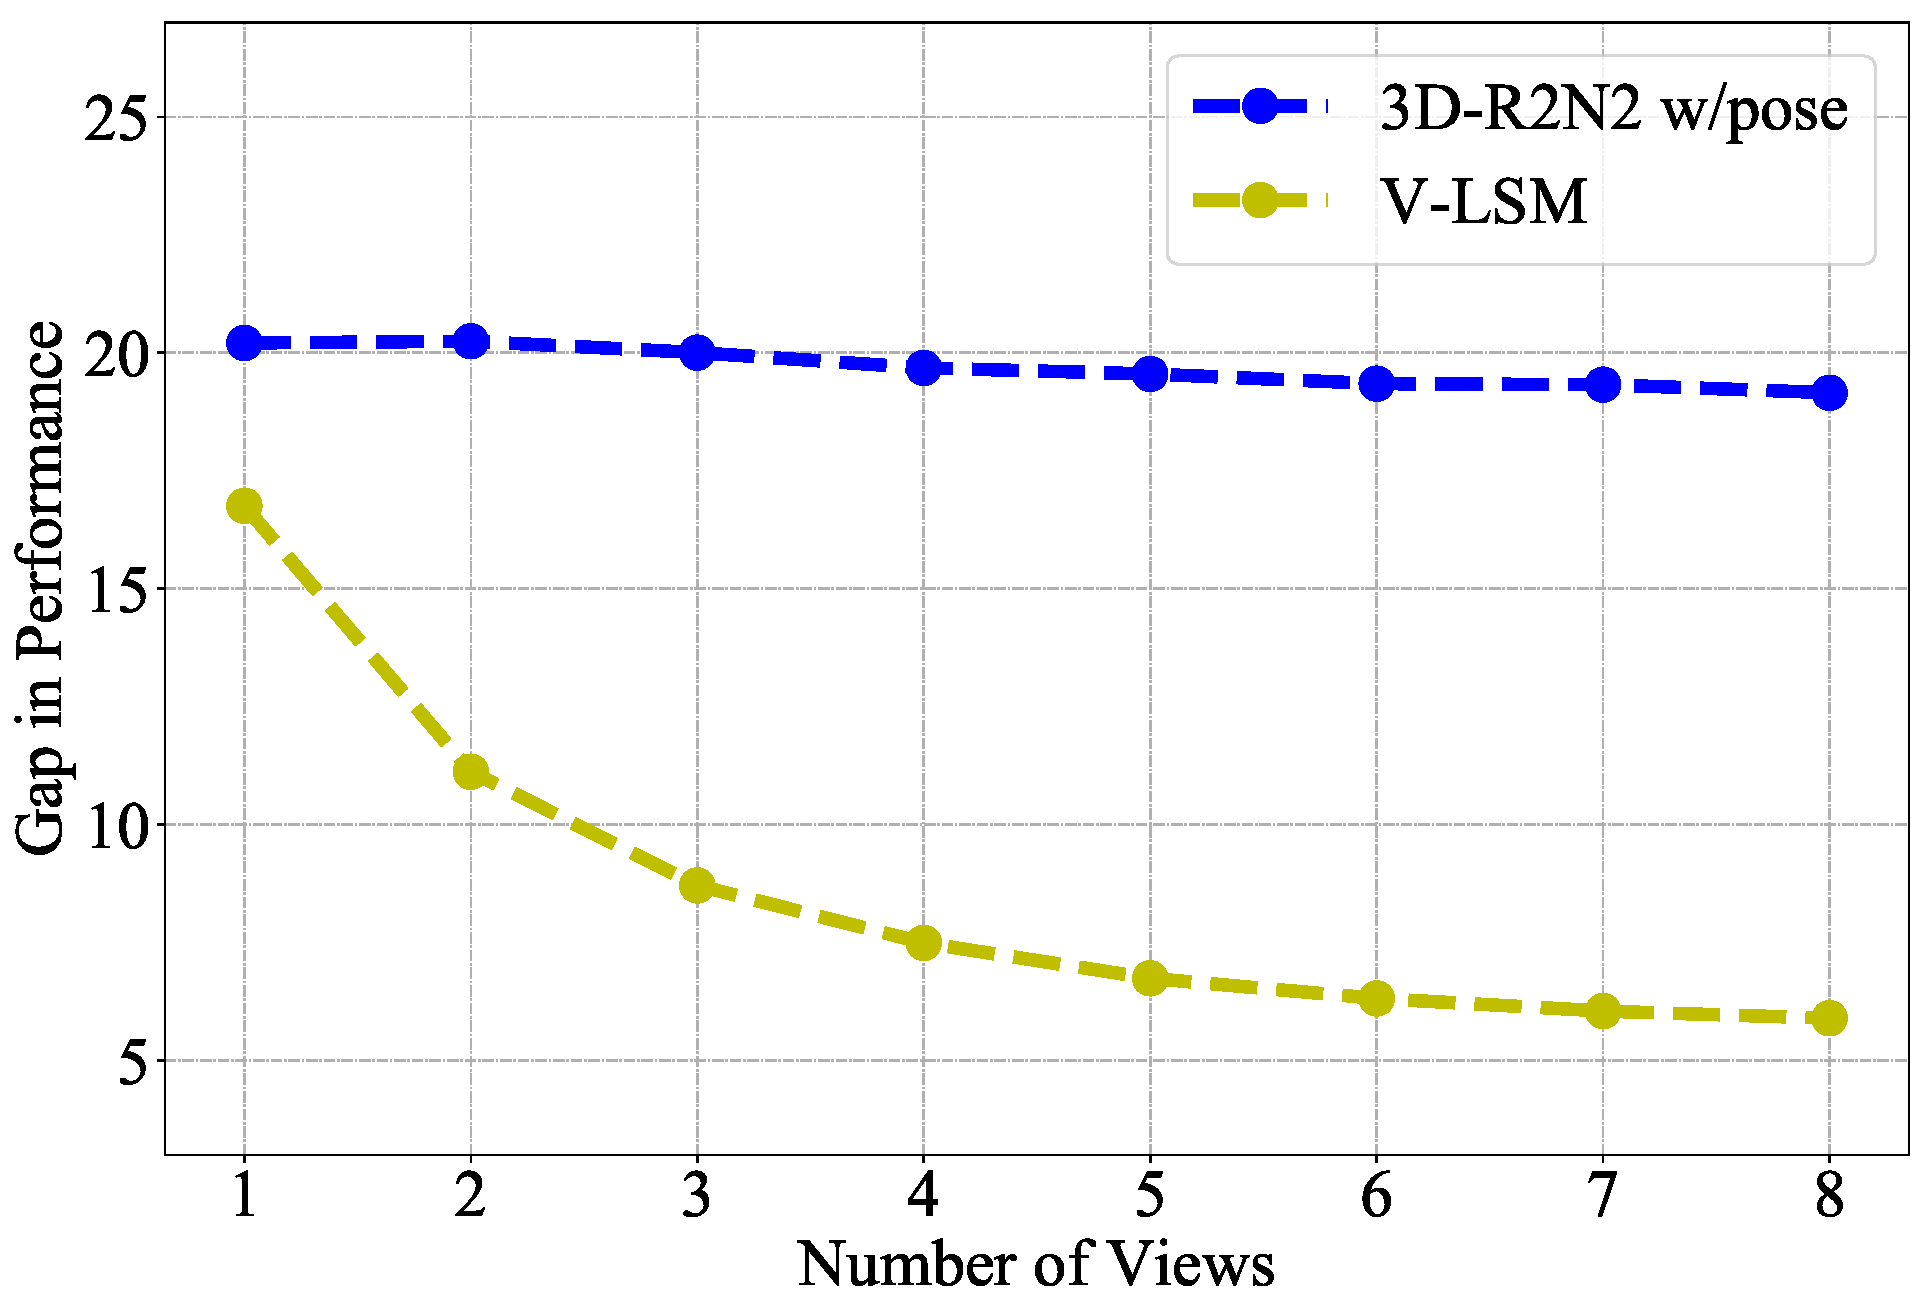
\includegraphics[width=0.6\linewidth]{figures/lsm/gen2.pdf}
\captionof{figure}{Generalization performance for V-LSM and 3D-R2N2 w/pose measured by gap in voxel IoU when tested on unseen object categories.}
\figlabel{generalization}
\end{figure}